\documentclass [xcolor=svgnames] {beamer} 
\usepackage[utf8]{inputenc}
\usepackage{xcolor}
\usepackage{booktabs, comment} 
\usepackage{pgfpages}
\usepackage{csquotes}
\usepackage{amsmath}
\usepackage{tikz}
\usetheme{Madrid}

% COLORS 
\definecolor{mqred}{RGB}{166, 25, 46}
\definecolor{mqdeepred}{RGB}{118, 35, 47}
\definecolor{mqgray}{RGB}{55, 58, 54}
\definecolor{mqlightgray}{RGB}{237, 235, 229}
\definecolor{mqmagenta}{RGB}{198, 0, 126}
\usecolortheme[named=mqred]{structure}
\setbeamercolor{title in head/foot}{bg=mqlightgray, fg=mqgray}
\setbeamercolor{author in head/foot}{bg=mqdeepred}
\setbeamercolor{page number in head/foot}{bg=mqdeepred, fg=mqlightgray}

% FOOTNOTE ARRANGEMENTS

\makeatletter
\setbeamertemplate{footline}{
	\leavevmode%
	\hbox{%
		\begin{beamercolorbox}[wd=.5\paperwidth,ht=2.25ex,dp=1ex,center]{author in head/foot}%
			\usebeamerfont{author in head/foot}\insertshortauthor\expandafter\ifblank\expandafter{\beamer@shortinstitute}{}{~~(\insertshortinstitute)}
		\end{beamercolorbox}%
		\begin{beamercolorbox}[wd=.4\paperwidth,ht=2.25ex,dp=1ex,center]{title in head/foot}%
			\usebeamerfont{title in head/foot}\insertshorttitle
		\end{beamercolorbox}%
		\begin{beamercolorbox}[wd=.1\paperwidth,ht=2.25ex,dp=1ex,center]{page number in head/foot}%
			\usebeamerfont{page number in head/foot}\insertframenumber{} / \inserttotalframenumber 
	\end{beamercolorbox}}%
	\vskip0pt%
}
\makeatother
\beamertemplatenavigationsymbolsempty


% TITLE, AUTHORS, INSTITUTE, DATE

\title[Short Title]{Caratterizzazione di un rivelatore gamma 4$\pi$ per lo studio della reazione 14N(p,$\gamma$)15O \\ \textit{Subtitle or Reference, if any}}
\author[P. Pusterla]{Paolo Pusterla}
\institute[UniTo]{Università degli Studi di Torino}
\date{6/7/8 Novembre 2024}

% LOGO
\titlegraphic{
\includegraphics[height=2.5cm]{img/logo.png}} % Change the logo path as needed

\begin{document}
	
	\begin{frame}
		\titlepage
	\end{frame}
	
	\begin{frame}{Outline}
		\tableofcontents
	\end{frame}
	
	% Section and Frame examples
	\section{Introduzione}
	\begin{frame}{L'esperimento}
		\begin{itemize}
			\item L'esperimento LUNA (Laboratory for Underground Nuclear Astrophysics) ricrea i processi nucleari che sono avvenuti durante la nucleosintesi primordiale e che avvengono tutt'ora nelle stelle.
			\item Essendo processi molto rari, un laboratorio sulla superficie terrestre non è adatto per le misure sperimentali di questi, poiché i raggi cosmici maschererebbero il segnale debole atteso.
			\item Per questo motivo i Laboratori Nazionali del Gran Sasso sono i luoghi adatti per questi esperimenti: le sale sperimentali in cui si effettuano sono protette e schermate dai 1400 m di roccia del monte Aquila. 
		\end{itemize}
	\end{frame}
	
	\begin{frame}{La reazione}
		\begin{itemize}
			\item Viene studiata la reazione $^{14}$N(p,$\gamma$)$^{15}$O del ciclo CNO, determinante per la produzione di neutrini solari.
			\item La misura della sezione d'urto di questa reazione ha portato alla riduzione di un fattore 2 del flusso di neutrini solari prodotti dal ciclo CNO.
			\item Ha inoltre permesso di aggiornare la stima dell'età della Via Lattea.
		\end{itemize}
	\end{frame}

	\begin{frame}{Il ciclo CNO}
		\begin{figure}[H]
			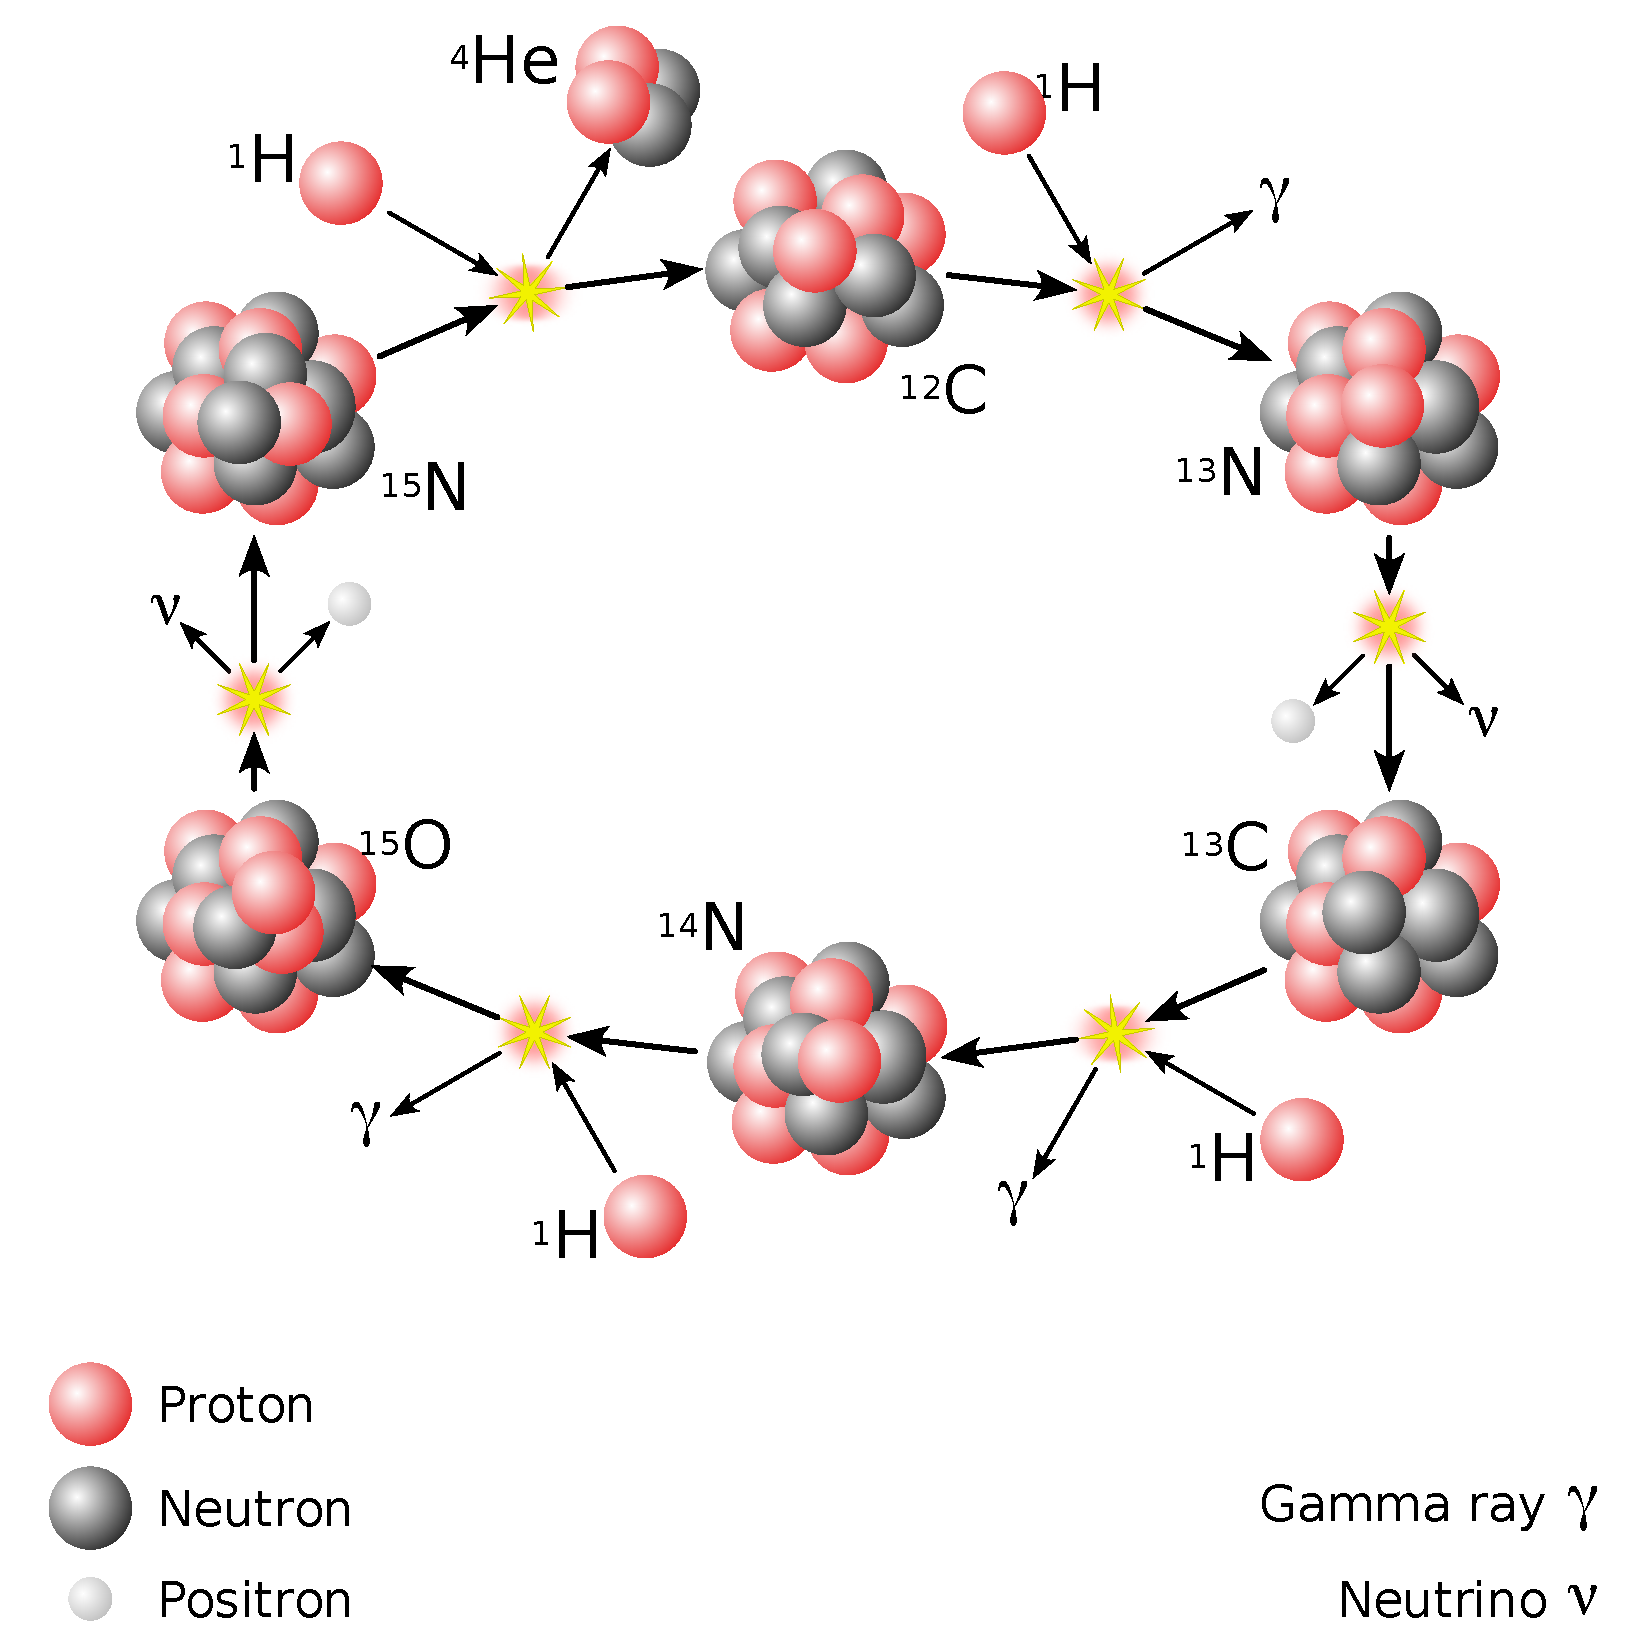
\includegraphics[width=0.5\textwidth]{img/CNO_Cycle.pdf}
			\caption{Ciclo Carbonio-Azoto-Ossigeno}
		\end{figure}
	\end{frame}

	\begin{frame}{L'acceleratore LUNA2 400 kV}
		\begin{itemize}
			\item Il fascio ionico utilizzato nell'esperimento è fornito dall'acceleratore elettrostatico LUNA2 a 400 kV.
			\item Installato nel 2001, ha soppiantato il precedente acceleratore di 50 kV (utilizzato sino al 2003) e fornisce fasci di ioni molto più intensi e temporalmente stabili.
		\end{itemize}
	\end{frame}
	
	\section{Obiettivi della tesi}
	\begin{frame}{Obiettivi}
		\begin{itemize}
			\item L'obiettivo della tesi è quello di caratterizzare in efficienza uno scintillatore $4\pi$ utilizzato per la rivelazione di raggi $\gamma$ nella riproduzione della reazione $^{14}$N(p,$\gamma$)$^{15}$O. 
			\item Include relevant equations, graphs, or figures.
		\end{itemize}
	\end{frame}
	
	\section{Il rivelatore}
	\begin{frame}{Il rivelatore $4\pi$}
		\begin{itemize}
			\item Lo scintillatore utilizzato è un rivelatore in germanato di bismuto (Bi$_{4}$Ge$_{3}$O$_{12}$, detto BGO).
			\item Il cristallo, di forma cilindrica, è otticamente separato in 6 spicchi diversi.
			\item I fotoni di scintillazione di ciascuno dei 6 segmenti sono rivelati da due fotomoltiplicatori.
		\end{itemize}
	\end{frame}

\begin{frame}{Il rivelatore $4\pi$}
	\begin{figure}[h]
		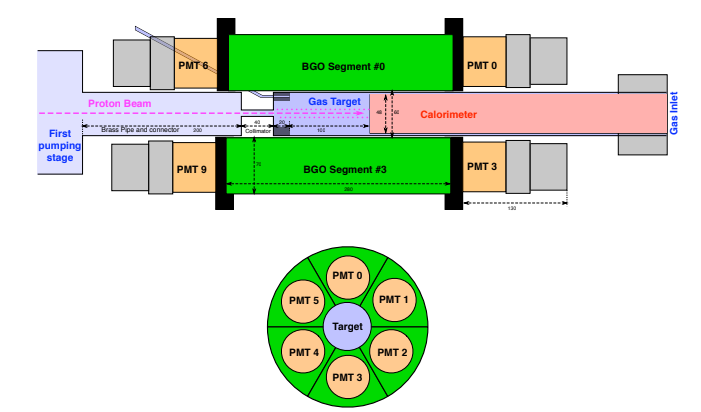
\includegraphics[width=0.8\textwidth]{img/BGO.png}
		\caption{Rappresentazione schematica del rivelatore BGO. In alto una sezione sagittale, in basso una sezione trasversale.}
	\end{figure}
\end{frame}

\section{Caratterizzaione}
\begin{frame}{Caratterizzazione in energia}
	\begin{itemize}
		\item La caratterizzazione in energia è effettuata utilizzando due sorgenti radioattive: Cobalto-60 e Cesio-137.
		\item Caratteristiche degli elementi utilizzati?
	\end{itemize}
\end{frame}
\begin{frame}
	\begin{itemize}
		\item I modi di decadimento degli elementi utilizzati sono
		\item Schema?? Energie che figurano nel nostro caso
	\end{itemize}
\end{frame}
\begin{frame}{Calcolo dell'efficienza}
	\begin{itemize}
		\item Per il calcolo dell'efficienza si possono applicare due metodi diversi
		\item Il primo metodo è geometrico, il secondo riguarda i parametri del fit sui picchi caratteristici.
		\item Il metodo geometrico trova applicazione nel cesio, ma poiché il cobalto presenta picchi sovrapposti, non è applicabile a quest'ultimo.
	\end{itemize}
\end{frame}
	
	\section{Conclusion}
	\begin{frame}{Conclusion}
		\begin{itemize}
			\item Summarize the key takeaways from your presentation.
			\item Mention any future work or open questions.
		\end{itemize}
	\end{frame}
	
	\begin{frame}
		\centering
		\textbf{Thank you!}\\
		Questions?
	\end{frame}
	
\end{document}

